\chapter{Inmunidad adaptativa y vacunación}\label{ch:b3:adaptive-immunity}

En 1796 un médico rural rascó pus de la llaga de viruela \omterm{def:b3:adaptive-immunity:vaccine}{vacuna} de una
ordeñadora y lo introdujo en el brazo de un niño, y seis semanas después
lo inoculó con viruela; el niño no enfermó. En 1980 la Organización
Mundial de la Salud declaró la viruela --- que había matado a trescientos
millones de personas en el siglo~XX --- erradicada de la Tierra con ese
método. El sistema que Jenner había reclutado, sin saber que existía,
puede reconocer cualquier molécula que jamás haya visto, elegir entre cien
mil millones de receptores distintos los pocos que encajan, multiplicar
por un millón en una semana las células que los llevan, mejorar su encaje
por mutación y selección mientras lo hace y recordar el resultado toda la
vida; además aprende a no atacar al cuerpo que lo fabricó, y sus fracasos
en aprenderlo son las enfermedades autoinmunitarias. Este capítulo trata
de los \omterm{def:b3:adaptive-immunity:lymphocytes}{linfocitos} y de cómo fabrican sus receptores, de cómo se monta y
se recuerda una respuesta, de cómo se impone y se pierde la \omterm{def:b3:adaptive-immunity:tolerance}{tolerancia}, y
de la aritmética por la que vacunar a bastante gente protege a la que no
lo está.

\section{Linfocitos y selección clonal}

\begin{definition}[Los linfocitos y sus receptores]\label{def:b3:adaptive-immunity:lymphocytes}
\index{linfocito}\index{linfocito B}\index{linfocito T}\index{antígeno}\index{selección clonal}\index{ganglio linfático}
La \emph{inmunidad adaptativa} la llevan los \emph{linfocitos}: los
\emph{linfocitos~B}, que maduran en la médula ósea y cuyo receptor de
antígeno es un \emph{\omterm{def:b3:adaptive-immunity:antibody}{anticuerpo}} anclado a la membrana que más tarde
secretan; y los \emph{linfocitos~T}, que maduran en el \omterm{def:b3:adaptive-immunity:tolerance}{timo} y cuyo
receptor reconoce fragmentos peptídicos expuestos en la superficie de
otras células. Un \emph{antígeno} es todo aquello que un receptor une; la
parte que se toca de hecho es un \emph{epítopo}. El hecho fundacional es
la \emph{selección clonal} (Burnet, 1957): cada linfocito lleva
receptores de una sola especificidad, fijada antes de encontrarse con
antígeno alguno; el cuerpo alberga un repertorio de unas $10^{11}$
células así; un antígeno selecciona a las pocas cuyos receptores encajan
y las empuja a dividirse en un clon de células efectoras y de memoria; y
los linfocitos cuyos receptores encajan con las moléculas propias del
cuerpo se eliminan o se silencian mientras maduran. Las células circulan
sin cesar entre la sangre y los \emph{ganglios linfáticos}, el bazo y el
tejido linfoide de las mucosas, donde se expone el antígeno que llevan
las \omterm{def:b3:innate-immunity:innate}{células dendríticas} (\cref{ch:b3:innate-immunity}), de modo que la
rara célula que encaja --- una de cada cien mil para un epítopo dado ---
lo encuentra en un día o dos.
\end{definition}

\begin{proof}[Evidencia]
Nossal y Lederberg (1958) colocaron \omterm{def:b3:adaptive-immunity:lymphocytes}{linfocitos} aislados de ratas
inmunizadas en microgotas y probaron el \omterm{def:b3:adaptive-immunity:antibody}{anticuerpo} que secretaba cada
uno: toda célula fabricaba \omterm{def:b3:adaptive-immunity:antibody}{anticuerpo} contra uno de los dos \omterm{def:b3:adaptive-immunity:lymphocytes}{antígenos},
nunca contra ambos. Burnet lo había predicho el año anterior. Tonegawa
(1976) comparó el ADN de un gen de \omterm{def:b3:adaptive-immunity:antibody}{anticuerpo} en células embrionarias y
en un \omterm{def:b3:cancer-biology:hallmarks}{tumor} secretor de \omterm{def:b3:adaptive-immunity:antibody}{anticuerpos}: en el embrión las partes variable y
constante estaban muy separadas, y en el \omterm{def:b3:cancer-biology:hallmarks}{tumor} estaban unidas --- el gen
había sido cortado y empalmado en la célula somática, la primera
demostración de un genoma reordenado a propósito.
\end{proof}

\section{Fabricar cien mil millones de receptores}

\begin{definition}[Estructura del anticuerpo y recombinación V(D)J]\label{def:b3:adaptive-immunity:antibody}
\index{anticuerpo}\index{inmunoglobulina}\index{recombinación V(D)J}\index{RAG}\index{diversidad de unión}\index{cambio de clase}
Un \emph{anticuerpo} (inmunoglobulina) son dos cadenas pesadas idénticas
y dos ligeras idénticas, cada una con un dominio \emph{variable} en su
extremo y dominios \emph{constantes} por detrás; cada uno de los dos
brazos une un epítopo mediante tres bucles hipervariables del dominio
variable pesado y tres del ligero, y el tallo (Fc) es lo que reconocen
los fagocitos, el \omterm{def:b3:innate-immunity:complement}{complemento} y los mastocitos. Cinco clases difieren en
la región constante de su cadena pesada: la IgM, la primera que se
fabrica, un pentámero que activa bien el \omterm{def:b3:innate-immunity:complement}{complemento}; la IgG, el caballo
de batalla de la sangre y los tejidos, que atraviesa la placenta; la IgA,
un dímero secretado a través de las superficies mucosas hacia el
intestino, las vías respiratorias y la leche; la IgE, que unen los
mastocitos, contra los gusanos --- y la causa de la alergia; y la IgD.
Los dominios variables no están codificados como tales. El locus de la
cadena pesada alberga unos $40$ segmentos \emph{V} funcionales, $25$
\emph{D} y $6$ \emph{J}; un linfocito~B en desarrollo elige uno de cada y
los une por \emph{recombinación V(D)J}: las enzimas RAG1 y RAG2 cortan en
las secuencias señal de recombinación que flanquean los segmentos, y los
extremos los une la maquinaria de \omterm{def:b3:dna-repair:dsb}{unión de extremos no homólogos} del
\cref{ch:b3:dna-repair}, con nucleótidos recortados y añadidos al azar
(por la enzima TdT) en cada juntura --- la \emph{diversidad de unión},
que cae exactamente en el tercer bucle hipervariable. Las cadenas ligeras
hacen lo mismo con V y J. Una vez iniciada la respuesta, ese mismo
dominio variable se une a una región constante distinta por un segundo
reordenamiento, el \emph{cambio de clase}, que cambia la función del
anticuerpo pero no su especificidad.
\end{definition}

\begin{theorem}[El tamaño del repertorio]\label{thm:b3:adaptive-immunity:repertoire}
\index{repertorio!combinatorio}
Con $V_{H} = 40$, $D = 25$ y $J_{H} = 6$ segmentos pesados, y cadenas
ligeras de dos loci con $(V_{\kappa}, J_{\kappa}) = (40, 5)$ y
$(V_{\lambda}, J_{\lambda}) = (30, 4)$, el número de combinaciones
distintas de pesada y ligera que se obtienen solo eligiendo segmentos es
\[
(40\times 25\times 6)\times(40\times 5 + 30\times 4) = 6000\times 320
= 1.9\times 10^{6}.
\]
La \omterm{def:b3:adaptive-immunity:antibody}{diversidad de unión} de las dos junturas pesadas y de la ligera
multiplica esto por un factor del orden de $10^{4}$--$10^{5}$, lo que da
un repertorio potencial por encima de $10^{10}$ a partir de menos de
$200$ segmentos génicos --- más que el número de linfocitos~B de un
cuerpo, de modo que el repertorio real es una muestra del posible. La
\omterm{def:b3:adaptive-immunity:germinal-centre}{hipermutación somática} durante la respuesta (más abajo) genera después
variantes de cada receptor seleccionado.
\end{theorem}
\begin{proof}
Cada cadena pesada es una V, una D y una J; cada cadena ligera, una V y
una J de cualquiera de los dos loci; y cualquier pesada se empareja con
cualquier ligera, de modo que los recuentos se multiplican (el principio
de multiplicación) y los dos loci ligeros se suman. El factor de unión es
el número de secuencias distintas que el recorte y la adición al azar
pueden producir en una juntura --- unas pocas decenas por juntura como
mínimo --- elevado al número de junturas; su valor exacto no está
definido, pero tres junturas con $30$ o $50$ resultados cada una dan de
$3\times 10^{4}$ a $10^{5}$. El recuento de los receptores de los
linfocitos~T, con dos cadenas reordenadas del mismo modo y una
contribución de unión mayor, es del mismo orden.
\end{proof}

\begin{omfigure}
\begin{tikzpicture}[every node/.style={font=\scriptsize}, >=stealth]
  % antibody Y
  \begin{scope}[xshift=0cm]
    % heavy chains
    \draw[very thick, omDef] (0,0) -- (0,1.6) -- (-1.3,3.0); \draw[very thick, omDef] (0.35,0) -- (0.35,1.6) -- (1.65,3.0);
    % light chains
    \draw[very thick, omProp] (-0.45,1.55) -- (-1.75,2.95); \draw[very thick, omProp] (0.8,1.55) -- (2.1,2.95);
    \fill[omThm] (-1.55,3.0) circle (0.12); \fill[omThm] (1.9,3.0) circle (0.12);
    \node[above, align=center] at (-1.5,3.15) {dominios variables:\\sitio de unión al antígeno}; 
    \node[right, align=left] at (0.55,0.5) {tallo Fc (constante):\\la clase decide la función};
    \node[left, omProp] at (-0.7,2.1) {ligera}; \node[right, omDef] at (0.4,1.3) {pesada};
    \draw[omDef] (0.05,1.1) -- (0.3,1.1); \draw[omDef] (0.05,0.7) -- (0.3,0.7);
  \end{scope}
  % V(D)J locus
  \begin{scope}[xshift=4.2cm, yshift=2.4cm, xscale=0.86]
    \draw[very thick, gray] (0,0) -- (8.2,0);
    \foreach \x in {0.2,0.6,1.0,1.4} \draw[thick, fill=omDef!40] (\x,-0.15) rectangle (\x+0.3,0.15);
    \node[above] at (0.95,0.2) {segmentos V ($\sim 40$)}; \node[font=\tiny] at (1.95,0) {$\cdots$};
    \foreach \x in {2.5,2.8,3.1} \draw[thick, fill=omProp!50] (\x,-0.15) rectangle (\x+0.2,0.15);
    \node[above] at (2.9,0.2) {D ($25$)};
    \foreach \x in {3.8,4.1,4.4} \draw[thick, fill=omMeth!50] (\x,-0.15) rectangle (\x+0.2,0.15);
    \node[above] at (4.2,0.2) {J ($6$)};
    \foreach \x/\lab in {5.3/\mu,6.0/\delta,6.7/\gamma,7.4/\alpha} { \draw[thick, fill=gray!30] (\x,-0.15) rectangle (\x+0.5,0.15); \node[above] at (\x+0.25,0.2) {C$_{\lab}$}; }
    \draw[->, thick] (4.1,-0.4) -- (4.1,-1.1) node[midway, right, align=left, font=\tiny] {RAG corta en las secuencias señal;\\se unen una V, una D y una J,\\y TdT añade nucleótidos al azar};
    % rearranged
    \draw[very thick, gray] (0,-1.5) -- (3.3,-1.5);
    \draw[thick, fill=omDef!40] (1.0,-1.65) rectangle (1.3,-1.35); \fill[omThm] (1.3,-1.65) rectangle (1.4,-1.35);
    \draw[thick, fill=omProp!50] (1.4,-1.65) rectangle (1.6,-1.35); \fill[omThm] (1.6,-1.65) rectangle (1.7,-1.35);
    \draw[thick, fill=omMeth!50] (1.7,-1.65) rectangle (1.9,-1.35);
    \draw[thick, fill=gray!30] (2.6,-1.65) rectangle (3.1,-1.35); \node[above] at (2.85,-1.3) {C$_{\mu}$};
    \node[below, align=center] at (1.45,-1.7) {VDJ unidos: el dominio variable;\\en rojo, los nucleótidos de unión};
    \node[right, align=left, font=\tiny] at (3.4,-2.0) {empalmado a C$_{\mu}$: una cadena pesada de IgM;\\el cambio de clase une después ese mismo\\VDJ a C$_{\gamma}$ o a C$_{\alpha}$};
  \end{scope}
\end{tikzpicture}

{\small Izquierda: un \omterm{def:b3:adaptive-immunity:antibody}{anticuerpo} --- dos cadenas pesadas y dos ligeras,
con los dominios variables en las puntas formando dos sitios de unión y
el tallo constante que lee el resto del sistema inmunitario. Derecha: el
locus de la cadena pesada antes y después de la \omterm{def:b3:adaptive-immunity:antibody}{recombinación V(D)J}, que
elige un segmento de cada clase y añade nucleótidos al azar en las
uniones.}
\end{omfigure}

\begin{definition}[Los receptores de los linfocitos~T y el MHC]\label{def:b3:adaptive-immunity:mhc}
\index{receptor del linfocito T}\index{complejo principal de histocompatibilidad}\index{presentación de antígenos}\index{restricción por MHC}\index{HLA}
El \emph{receptor del linfocito~T} es una molécula de dos cadenas
construida por la misma recombinación, que nunca se secreta y que no une
\omterm{def:b3:adaptive-immunity:lymphocytes}{antígeno} libre en disolución: reconoce un péptido corto alojado en el
surco de una molécula del \emph{complejo principal de
histocompatibilidad} (MHC) de la superficie de otra célula. El \emph{MHC
de clase~I}, presente en toda célula nucleada, expone péptidos de ocho a
diez residuos que el proteasoma ha cortado de las proteínas citosólicas
de la propia célula --- una muestra de lo que la célula está fabricando,
\omterm{def:b3:virology:virus}{virus} incluido --- a los linfocitos~T \emph{CD8}, que matan a la célula
si el péptido es ajeno. El \emph{MHC de clase~II}, presente en \omterm{def:b3:innate-immunity:innate}{células
dendríticas}, \omterm{def:b3:innate-immunity:innate}{macrófagos} y linfocitos~B, expone péptidos de trece a
veinticinco residuos de proteínas que la célula ha captado y digerido en
\omterm{def:b3:membrane-traffic:endocytosis}{endosomas}, a los linfocitos~T \emph{CD4}, que responden ayudando. Un
linfocito~T está \emph{restringido}: reconoce su péptido solo sobre el
alelo del MHC con el que fue seleccionado. Los genes del MHC (el
\emph{HLA} en el ser humano) son los más polimórficos del genoma, con
miles de alelos que difieren cada uno en el surco, de modo que cada
persona expone una muestra distinta de los péptidos de cada proteína y
ningún patógeno puede escapar a la presentación en todo el mundo --- y de
modo que un órgano trasplantado de un donante no compatible lo reconoce
como ajeno una gran parte de los linfocitos~T del receptor.
\end{definition}

\begin{proof}[Evidencia]
Zinkernagel y Doherty (1974) infectaron con un \omterm{def:b3:virology:virus}{virus} ratones de dos cepas
consanguíneas y probaron sus linfocitos~T citotóxicos sobre células diana
infectadas: los linfocitos~T mataban a las células infectadas de su
propia cepa pero no a las de la otra, aunque el \omterm{def:b3:virology:virus}{virus} fuera el mismo. El
linfocito~T veía el \omterm{def:b3:virology:virus}{virus} solo junto a una molécula propia del MHC --- la
\emph{\omterm{def:b3:adaptive-immunity:mhc}{restricción por MHC}} ---, algo que se explicó más tarde cuando la
estructura cristalina de una molécula del MHC (Bjorkman, 1987) mostró un
surco con un péptido dentro, y se demostró que el receptor del
linfocito~T une a los dos juntos.
\end{proof}

\begin{omfigure}
\begin{tikzpicture}[every node/.style={font=\scriptsize}, >=stealth]
  % class I pathway
  \begin{scope}
    \draw[thick, omDef, fill=omDef!8] (0,0) rectangle (6.2,3.6); \node[anchor=north west] at (0.05,3.55) {cualquier célula nucleada};
    \node[draw, rounded corners, fill=omThm!20, font=\tiny, align=center] (v) at (1.4,2.6) {proteína vírica o propia\\en el citosol};
    \node[draw, rounded corners, fill=gray!20, font=\tiny, align=center] (p) at (1.4,1.5) {proteasoma:\\péptidos de 8--10};
    \node[draw, rounded corners, fill=omDef!25, font=\tiny, align=center] (er) at (4.6,1.5) {RE: cargados en\\el MHC de clase I};
    \draw[->, thick] (v) -- (p); \draw[->, thick] (p) -- node[midway, above, font=\tiny] {TAP} (er);
    \draw[->, thick] (er) -- (4.6,3.55);
    \draw[thick, fill=omDef!40] (4.4,3.6) rectangle (4.8,4.1); \fill[omThm] (4.6,4.2) circle (0.09);
    \node[above, align=center] at (4.6,4.35) {péptido--MHC I\\visto por linfocitos T CD8: matan};
  \end{scope}
  % class II pathway
  \begin{scope}[xshift=7.2cm]
    \draw[thick, omProp, fill=omProp!8] (0,0) rectangle (6.2,3.6); \node[anchor=north west] at (0.05,3.55) {célula dendrítica, macrófago, linfocito B};
    \node[draw, rounded corners, fill=omThm!20, font=\tiny, align=center] (ex) at (1.4,2.6) {proteína captada\\en un endosoma};
    \node[draw, rounded corners, fill=gray!20, font=\tiny, align=center] (dig) at (1.4,1.5) {digerida:\\péptidos de 13--25};
    \node[draw, rounded corners, fill=omProp!30, font=\tiny, align=center] (m2) at (4.6,1.5) {MHC de clase II\\cargado aquí};
    \draw[->, thick] (ex) -- (dig); \draw[->, thick] (dig) -- (m2);
    \draw[->, thick] (m2) -- (4.6,3.55);
    \draw[thick, fill=omProp!50] (4.4,3.6) rectangle (4.8,4.1); \fill[omThm] (4.6,4.2) circle (0.09);
    \node[above, align=center] at (4.6,4.35) {péptido--MHC II\\visto por linfocitos T CD4: ayudan};
  \end{scope}
\end{tikzpicture}

{\small Las dos vías de presentación. La clase~I muestra a los
linfocitos~T CD8 lo que una célula está fabricando en su interior; la
clase~II muestra a los linfocitos~T CD4 lo que una célula presentadora ha
comido. Una respuesta citotóxica se dirige a la primera, y una respuesta
de ayuda a la segunda.}
\end{omfigure}

\section{La respuesta}

\begin{definition}[Activación, ayuda y muerte]\label{def:b3:adaptive-immunity:response}
\index{linfocito T colaborador}\index{linfocito T citotóxico}\index{coestimulación}\index{linfocito T regulador}\index{célula plasmática}\index{célula de memoria}
Un linfocito~T virgen se activa cuando su receptor une péptido--MHC en
una \omterm{def:b3:innate-immunity:innate}{célula dendrítica} que además aporta coestimulación
(\cref{ch:b3:innate-immunity}); entonces se divide cada seis u ocho horas
durante una semana y se diferencia. Los linfocitos~T \emph{CD4
colaboradores} se diferencian, según las \omterm{def:b3:innate-immunity:inflammation}{citocinas} de la \omterm{def:b3:innate-immunity:innate}{célula
dendrítica}, en subconjuntos: Th1, que activan a los \omterm{def:b3:innate-immunity:innate}{macrófagos} para que
maten lo que han comido (la tuberculosis); Th2, que impulsan la IgE y los
eosinófilos contra los gusanos; Th17, que reclutan \omterm{def:b3:innate-immunity:innate}{neutrófilos} contra
bacterias y hongos extracelulares; los colaboradores foliculares, que
ayudan a los linfocitos~B; y los linfocitos~T \emph{reguladores}, que
suprimen. Los linfocitos~T \emph{CD8 citotóxicos} matan a las células que
exponen su péptido en la clase~I, con perforina y granzimas y con el
ligando de Fas, y desencadenan la \omterm{def:b3:cell-cycle-apoptosis:apoptosis}{apoptosis}
(\cref{ch:b3:cell-cycle-apoptosis}) --- la defensa contra los \omterm{def:b3:virology:virus}{virus} y los
\omterm{def:b3:cancer-biology:hallmarks}{tumores}. Un linfocito~B se activa por la unión del \omterm{def:b3:adaptive-immunity:lymphocytes}{antígeno} a su receptor
más la ayuda de un linfocito~T colaborador folicular que reconozca
péptidos de ese mismo \omterm{def:b3:adaptive-immunity:lymphocytes}{antígeno} en la clase~II del linfocito~B; se
convierte entonces en una \emph{célula plasmática} que secreta miles de
\omterm{def:b3:adaptive-immunity:antibody}{anticuerpos} por segundo, durante días (las de vida corta, en el ganglio)
o durante años (las de vida larga, en la médula), o entra en un \omterm{def:b3:adaptive-immunity:germinal-centre}{centro
germinal}. Los linfocitos~B y T de \emph{memoria} --- longevos, más
numerosos que los precursores vírgenes y más rápidos en responder --- son
el residuo de toda respuesta y la base de la vacunación.
\end{definition}

\begin{definition}[El centro germinal]\label{def:b3:adaptive-immunity:germinal-centre}
\index{centro germinal}\index{hipermutación somática}\index{maduración de la afinidad}
En un \emph{centro germinal}, una estructura que se forma en un \omterm{def:b3:adaptive-immunity:lymphocytes}{ganglio
linfático} hacia la primera semana de una respuesta, los linfocitos~B
activados ejecutan un algoritmo evolutivo. En su zona oscura se dividen
cada seis horas y la enzima AID muta los genes variables de su \omterm{def:b3:adaptive-immunity:antibody}{anticuerpo}
a razón de un cambio por cada mil pares de bases y división --- la
\emph{hipermutación somática}, un millón de veces la tasa genómica y
dirigida a una kilobase. En la zona clara cada célula prueba su nuevo
receptor contra el \omterm{def:b3:adaptive-immunity:lymphocytes}{antígeno} que retienen las \omterm{def:b3:innate-immunity:innate}{células dendríticas}
foliculares y compite por la ayuda de los linfocitos~T: las células que
unen mejor captan más \omterm{def:b3:adaptive-immunity:lymphocytes}{antígeno}, presentan más, reciben más ayuda y
vuelven a la zona oscura a dividirse otra vez; las que unen peor, o que
han perdido la unión, mueren por \omterm{def:b3:cell-cycle-apoptosis:apoptosis}{apoptosis}. A lo largo de dos o tres
semanas de ciclos, la afinidad de los \omterm{def:b3:adaptive-immunity:antibody}{anticuerpos} supervivientes sube de
cien a mil veces --- la \emph{maduración de la afinidad} --- y las
ganadoras se marchan como \omterm{def:b3:adaptive-immunity:response}{células plasmáticas} y \omterm{def:b3:adaptive-immunity:response}{células de memoria}, tras
haber cambiado además de clase. La respuesta secundaria es más rápida,
mayor y de mejor \omterm{def:b3:adaptive-immunity:antibody}{anticuerpo} porque parte de esa población seleccionada,
expandida y cambiada de clase.
\end{definition}

\begin{omfigure}
\begin{tikzpicture}[every node/.style={font=\scriptsize}, >=stealth]
  \draw[thick, omDef, fill=omDef!12] (0,0) ellipse (2.7 and 1.7); \node[above, omDef!70!black] at (0,1.75) {zona oscura};
  \draw[thick, omMeth!70!black, fill=omMeth!12] (6.2,0) ellipse (2.7 and 1.7); \node[above, omMeth!60!black] at (6.2,1.75) {zona clara};
  \node[align=center] at (0,0.3) {los linfocitos B se dividen cada \qty{6}{h};\\AID muta los genes del anticuerpo:\\$10^{-3}$ por bp y división};
  \node[align=center] at (6.2,0.3) {prueban el nuevo receptor\\sobre el antígeno que retienen\\las células dendríticas foliculares;\\compiten por la ayuda de los linfocitos T};
  \draw[->, very thick, omProp] (2.4,0.7) .. controls (3.6,1.4) and (4.2,1.4) .. (3.7,0.7); \node[above, omProp] at (3.1,1.45) {salen los mutantes};
  \draw[->, very thick, omMeth!70!black] (3.7,-0.7) .. controls (4.2,-1.4) and (3.6,-1.4) .. (2.4,-0.7); \node[below, omMeth!70!black] at (3.1,-1.45) {vuelven las ganadoras, a dividirse otra vez};
  \draw[->, thick, omThm] (6.6,-1.6) -- (6.6,-2.3); \node[below, omThm, align=center] at (6.6,-2.3) {perdedoras: apoptosis\\(casi todas)};
  \draw[->, thick] (8.9,0) -- (9.5,0); \node[right, align=left] at (9.5,0) {tras 2 o 3 semanas:\\células plasmáticas\\(longevas, en la médula)\\y linfocitos B de memoria;\\afinidad $100$--$1000\times$\\mayor, con clase cambiada};
\end{tikzpicture}

{\small El \omterm{def:b3:adaptive-immunity:germinal-centre}{centro germinal} como máquina evolutiva: mutación en la zona
oscura, selección en la zona clara y ciclos entre ambas hasta que los
\omterm{def:b3:adaptive-immunity:antibody}{anticuerpos} que salen unen mucho mejor que los que entraron.}
\end{omfigure}

\begin{example}[Cinética de una respuesta]\label{ex:b3:adaptive-immunity:kinetics}
Alrededor de un linfocito~B de cada $10^{5}$ une un epítopo dado, de modo
que los $10^{11}$ linfocitos~B de un cuerpo contienen unos $10^{6}$
precursores, de los que quizá un centenar se encuentre con el \omterm{def:b3:adaptive-immunity:lymphocytes}{antígeno} en
el ganglio que drena la zona. Dividiéndose cada ocho horas, cien células
se convierten en $10^{2}\times 2^{21} \approx 2\times 10^{8}$ en una
semana. El \omterm{def:b3:adaptive-immunity:antibody}{anticuerpo} aparece en el suero al cabo de cuatro a seis días,
primero la IgM, alcanza su máximo hacia las dos semanas y decae con una
semivida de tres semanas para la IgG a medida que mueren las \omterm{def:b3:adaptive-immunity:response}{células
plasmáticas} de vida corta, hasta asentarse en el nivel que mantienen
durante años las \omterm{def:b3:adaptive-immunity:response}{células plasmáticas} longevas de la médula. Una segunda
exposición parte de $10^{4}$--$10^{5}$ \omterm{def:b3:adaptive-immunity:response}{células de memoria} de alta
afinidad ya cambiadas a IgG: el \omterm{def:b3:adaptive-immunity:antibody}{anticuerpo} sube en dos días, de diez a
cien veces más alto, y neutraliza al patógeno antes de que pueda
asentarse --- que es lo que compra una \omterm{def:b3:adaptive-immunity:vaccine}{vacuna}.
\end{example}

\begin{omfigure}
\begin{tikzpicture}
\begin{axis}[
  width=0.7\linewidth, height=5.6cm,
  axis x line=bottom, axis y line=left,
  xmin=0, xmax=70, ymin=1, ymax=10000, ymode=log,
  xlabel={días}, ylabel={anticuerpo sérico (relativo)},
  xlabel style={font=\small, at={(axis description cs:0.5,-0.12)}, anchor=north}, ylabel style={font=\small},
  tick label style={font=\small}, xtick={0,10,20,30,40,50,60,70},
  clip=false,
]
\addplot[very thick, omDef, domain=0:40, samples=60] {1 + 100*exp(-((x-14)/5)^2) + 15*(1-exp(-x/10))*exp(-(x-14)/60)*(x>14)};
\addplot[very thick, omThm, domain=40:70, samples=60] {1 + 2500*exp(-((x-48)/5)^2) + 400*(1-exp(-(x-40)/4))*(x>40)};
\draw[->, thick, gray] (axis cs:0,0.6) -- (axis cs:0,1.8); \node[font=\scriptsize, gray, anchor=south west] at (axis cs:0.5,1.3) {primera exposición};
\draw[->, thick, gray] (axis cs:40,0.6) -- (axis cs:40,1.8); \node[font=\scriptsize, gray, anchor=south west] at (axis cs:40.5,1.3) {segunda exposición};
\node[font=\scriptsize, omDef, anchor=south west] at (axis cs:2,600) {primaria: IgM y luego IgG, máximo a las dos semanas};
\node[font=\scriptsize, omThm, anchor=south east] at (axis cs:69,3500) {secundaria: más rápida, más alta, IgG, más afinidad};
\end{axis}
\end{tikzpicture}

{\small Respuestas de \omterm{def:b3:adaptive-immunity:antibody}{anticuerpos} primaria y secundaria. La segunda
exposición parte de una población de memoria expandida, con clase
cambiada y afinidad madurada, y responde en días a un nivel que la
primera respuesta nunca alcanzó.}
\end{omfigure}

\begin{omfigure}
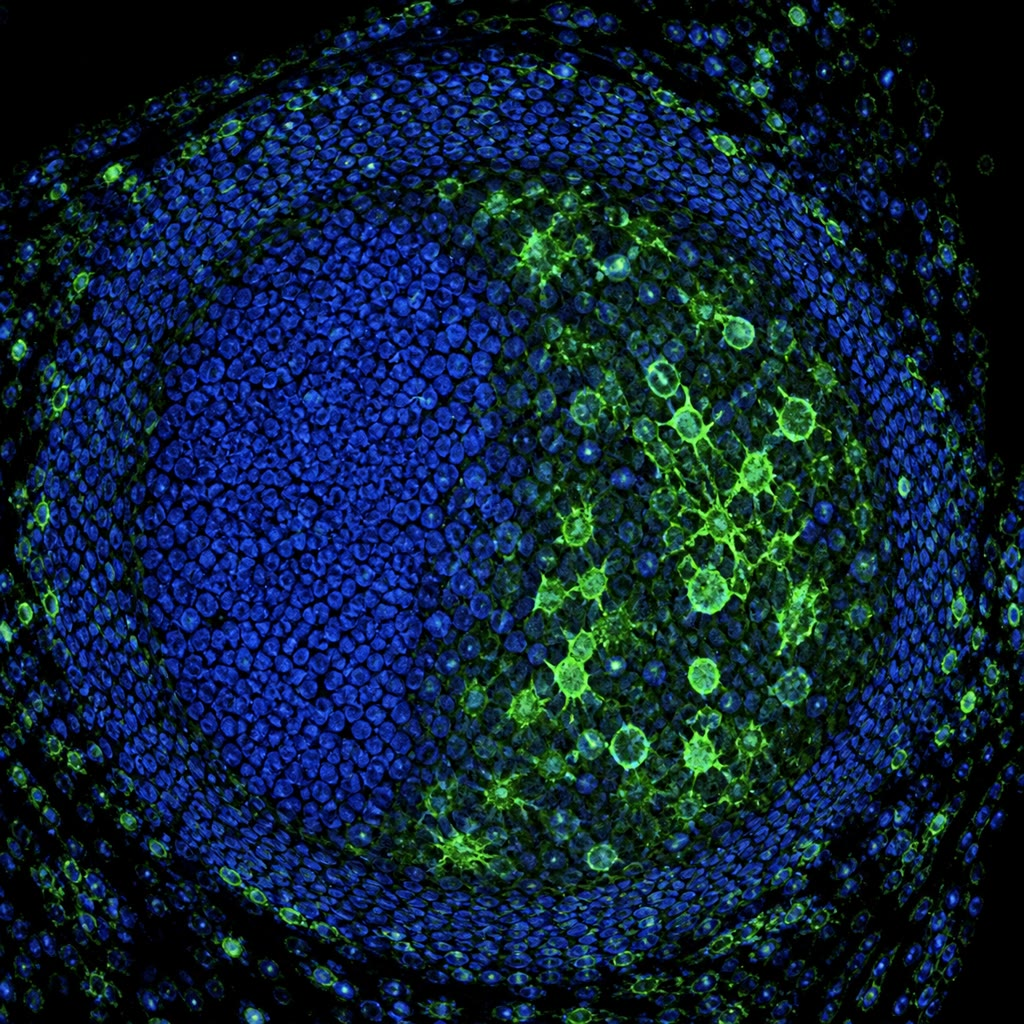
\includegraphics[width=0.36\linewidth]{images/book5/ai/b5-16-germinal-centre.jpg}\hspace{0.04\linewidth}
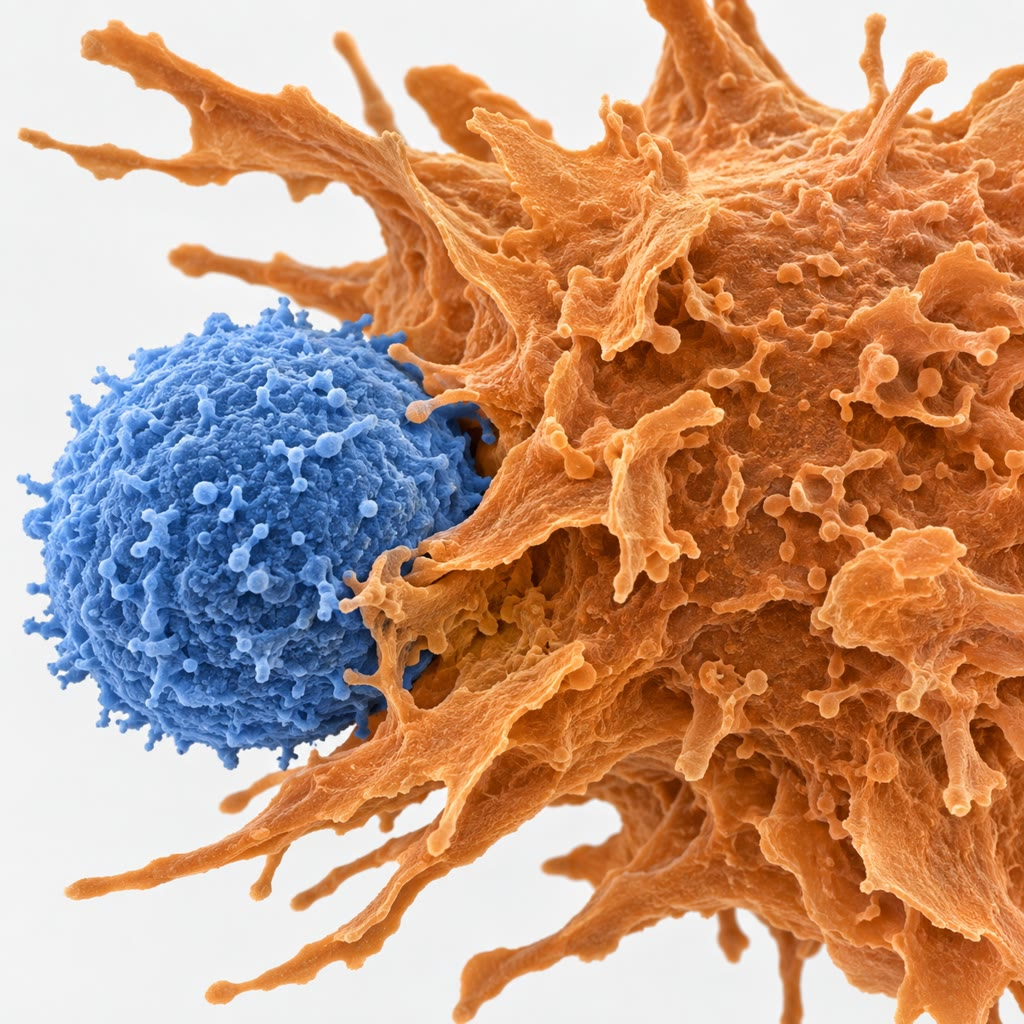
\includegraphics[width=0.36\linewidth]{images/book5/ai/b5-16-t-cell-apc.jpg}

{\small Izquierda: un \omterm{def:b3:adaptive-immunity:germinal-centre}{centro germinal} en un \omterm{def:b3:adaptive-immunity:lymphocytes}{ganglio linfático} --- la
apretada zona oscura y la zona más clara de la selección. Derecha: un
linfocito~T (pequeño) en contacto con una \omterm{def:b3:innate-immunity:innate}{célula dendrítica}, el momento
en que se decide la respuesta adaptativa.}
\end{omfigure}

\section{La tolerancia y sus fracasos}

\begin{definition}[Tolerancia]\label{def:b3:adaptive-immunity:tolerance}
\index{tolerancia}\index{selección negativa}\index{timo}\index{anergia}\index{FoxP3}\index{autoinmunidad}
El repertorio se fabrica al azar y contiene por tanto receptores para lo
propio. La \emph{tolerancia central} los elimina allí donde maduran las
células: en el timo se matan los linfocitos~T cuyos receptores unen con
demasiada fuerza el péptido--MHC propio (la \emph{selección negativa}),
se matan también los que no pueden unir el MHC en absoluto (serían
inútiles) y solo sale el escaso porcentaje intermedio; un factor de
transcripción, AIRE, hace que las células tímicas expresen proteínas de
todos los tejidos --- insulina, tiroglobulina --- para que allí puedan
eliminarse los linfocitos~T específicos de ellas. Los linfocitos~B que
unen lo propio en la médula se eliminan o editan sus receptores. La
\emph{tolerancia periférica} se ocupa del resto: un linfocito~T que se
encuentra con su \omterm{def:b3:adaptive-immunity:lymphocytes}{antígeno} sin \omterm{def:b3:adaptive-immunity:response}{coestimulación} queda incapaz de responder
(la \emph{anergia}) o se elimina; y los linfocitos~T \emph{reguladores},
definidos por el factor FoxP3, suprimen activamente las respuestas contra
lo propio y contra \omterm{def:b3:adaptive-immunity:lymphocytes}{antígenos} inocuos como los alimentos y los comensales.
La \emph{autoinmunidad} es el fracaso de estos controles: la diabetes de
tipo~1 (los linfocitos~T destruyen las células $\beta$), la esclerosis
múltiple (la mielina), la artritis reumatoide (las articulaciones), el
lupus (\omterm{def:b3:adaptive-immunity:antibody}{anticuerpos} contra componentes nucleares), la enfermedad
tiroidea; cada una se asocia a alelos \omterm{def:b3:adaptive-immunity:mhc}{HLA} concretos, que presentan los
péptidos propios pertinentes, y algunas las desencadena la infección por
un microbio cuyos péptidos se parecen a una proteína propia (la fiebre
reumática tras una infección estreptocócica).
\end{definition}

\begin{proof}[Evidencia]
Medawar (1953) inyectó células de una cepa consanguínea de ratón en
ratones recién nacidos de otra; ya adultos, los receptores aceptaban
injertos de piel de la cepa donante que de otro modo habrían rechazado,
mientras rechazaban los injertos de terceras cepas. La \omterm{def:b3:adaptive-immunity:tolerance}{tolerancia} era
adquirida, específica y fijada por aquello con lo que el sistema
inmunitario se había encontrado pronto --- la base experimental de la
eliminación de clones autorreactivos de Burnet. Los niños que nacen sin
un gen AIRE funcional desarrollan \omterm{def:b3:adaptive-immunity:tolerance}{autoinmunidad} contra muchos órganos a
la vez; los que no tienen \omterm{def:b3:adaptive-immunity:tolerance}{FoxP3} (un síndrome raro ligado al X)
desarrollan una \omterm{def:b3:adaptive-immunity:tolerance}{autoinmunidad} mortal en la lactancia --- los dos brazos
de la \omterm{def:b3:adaptive-immunity:tolerance}{tolerancia}, mostrado cada uno por su ausencia.
\end{proof}

\begin{example}[Hipersensibilidad, deficiencia, trasplante]\label{ex:b3:adaptive-immunity:failures}
La \emph{alergia} es una respuesta Th2 a un \omterm{def:b3:adaptive-immunity:lymphocytes}{antígeno} inocuo --- polen,
cacahuete, penicilina --- que produce IgE; al reexponerse, el \omterm{def:b3:adaptive-immunity:lymphocytes}{antígeno}
entrecruza la IgE de los mastocitos, que liberan histamina en cuestión de
minutos, y si el \omterm{def:b3:adaptive-immunity:lymphocytes}{antígeno} está en la sangre la liberación sistémica es la
\emph{anafilaxia}, que se trata con adrenalina. La
\emph{inmunodeficiencia}: los niños que carecen de \omterm{def:b3:adaptive-immunity:antibody}{RAG} o de la enzima ADA
no fabrican \omterm{def:b3:adaptive-immunity:lymphocytes}{linfocitos} (la inmunodeficiencia combinada grave) y mueren de
infección si no reciben médula o terapia génica; el VIH destruye los
linfocitos~T CD4 y con ellos la ayuda que toda respuesta necesita. El
\emph{trasplante}: los linfocitos~T del receptor ven como ajenas las
moléculas \omterm{def:b3:adaptive-immunity:mhc}{HLA} del donante, y hasta una décima parte de todos los
linfocitos~T responden --- mucho más que a cualquier patógeno ---, de
modo que los injertos se emparejan en los loci \omterm{def:b3:adaptive-immunity:mhc}{HLA} y el receptor queda
inmunodeprimido de por vida; un injerto de médula puede, al revés,
atacar a su nuevo hospedador. Y los usos deliberados: los \omterm{def:b3:genetic-engineering:expression}{anticuerpos
monoclonales} del \cref{ch:b3:genetic-engineering}, los \omterm{prop:b3:cancer-biology:immune}{inhibidores de
puntos de control} que sueltan a los linfocitos~T contra los \omterm{def:b3:cancer-biology:hallmarks}{tumores}
(\cref{ch:b3:cancer-biology}) y los linfocitos~T dotados por ingeniería
de un receptor quimérico para un \omterm{def:b3:adaptive-immunity:lymphocytes}{antígeno} tumoral (las CAR-T), que han
curado leucemias que ninguna otra cosa tocaba.
\end{example}

\section{La vacunación}

\begin{definition}[Vacunas e inmunidad de grupo]\label{def:b3:adaptive-immunity:vaccine}
\index{vacuna}\index{inmunidad de grupo}\index{número reproductivo básico}\index{eficacia vacunal}
Una \emph{vacuna} presenta \omterm{def:b3:adaptive-immunity:lymphocytes}{antígenos} de un patógeno, con un adyuvante o
en una forma que dispare los receptores innatos, de manera que quien la
recibe adquiere \omterm{def:b3:adaptive-immunity:response}{células de memoria} y \omterm{def:b3:adaptive-immunity:antibody}{anticuerpos} sin la enfermedad (el
\cref{ch:b3:virology} enumera las clases). Su \emph{eficacia} $E$ es la
fracción de vacunados que quedan protegidos. La protección se extiende
más allá de los vacunados: un patógeno que se propaga en una población en
la que cada caso infecta a otros $R_{0}$ en promedio cuando todos son
susceptibles --- el \emph{número reproductivo básico} --- infecta solo a
$R_{0}$ veces la fracción susceptible cuando algunos son inmunes, y se
extingue cuando ese número baja de uno. Esto es la \emph{inmunidad de
grupo}: por encima de un umbral de personas inmunes, la cadena de
transmisión se rompe y los no vacunados --- los lactantes, los
inmunodeprimidos, aquellos en quienes la vacuna falló --- quedan
protegidos por los demás.
\end{definition}

\begin{theorem}[El umbral de la inmunidad de grupo]\label{thm:b3:adaptive-immunity:herd}
\index{inmunidad de grupo!umbral}\index{modelo SIR}
En una población en la que una fracción $p$ es inmune y el resto
susceptible, cada caso infecta en promedio a otros
$R_{\text{ef}} = R_{0}(1 -
p)$. Una epidemia no puede arrancar si $R_{\text{ef}} < 1$, es decir, si
\[
p > p_{c} = 1 - \frac{1}{R_{0}} .
\]
Con una \omterm{def:b3:adaptive-immunity:vaccine}{vacuna} de eficacia $E$, la cobertura necesaria es
$f_{c} = p_{c}/E$. Si una epidemia llega a correr en una población
susceptible (el \omterm{thm:b3:adaptive-immunity:herd}{modelo SIR}, con tasa de infección $\beta$ y tasa de
recuperación $\gamma$, $R_{0} =
\beta/\gamma$), alcanza su máximo cuando la fracción susceptible ha caído
a $1/R_{0}$, y la fracción que nunca se infecta, $s_{\infty}$, cumple
$\ln s_{\infty} = -R_{0}(1 - s_{\infty})$.
\end{theorem}
\begin{proof}
Cada caso establece contactos que infectarían a $R_{0}$ personas si todas
fueran susceptibles; lo es una fracción $1 - p$ de ellas, de modo que
$R_{\text{ef}} =
R_{0}(1-p)$, y la condición $R_{\text{ef}} < 1$ da $p_{c}$; una \omterm{def:b3:adaptive-immunity:vaccine}{vacuna}
que protege a una fracción $E$ de quienes la reciben vuelve inmune a una
fracción $Ef$ de la población, luego $Ef > p_{c}$. En el \omterm{thm:b3:adaptive-immunity:herd}{modelo SIR},
$\mathrm{d}s/\mathrm{d}t = -\beta si$ y $\mathrm{d}i/\mathrm{d}t =
\beta si - \gamma i = \gamma i(R_{0}s - 1)$, de modo que $i$ crece
mientras $s >
1/R_{0}$ y cae después: el máximo está en $s = 1/R_{0}$. Dividiendo las
dos ecuaciones, $\mathrm{d}i/\mathrm{d}s = -1 + 1/(R_{0}s)$, de modo que
$i + s -
\ln s/R_{0}$ es constante; evaluándolo al principio ($s = 1$, $i
\approx 0$) y al final ($i = 0$, $s = s_{\infty}$) resulta
$s_{\infty} - \ln s_{\infty}/R_{0} = 1$, la relación del tamaño final.
\end{proof}

\begin{example}[Sarampión y viruela]\label{ex:b3:adaptive-immunity:measles}
El sarampión tiene $R_{0} \approx 15$: $p_{c} = 1 - 1/15 = 93\,\%$ y, con
una \omterm{def:b3:adaptive-immunity:vaccine}{vacuna} de eficacia $97\,\%$ tras dos dosis, la cobertura necesaria es
del $96\,\%$ --- que es por lo que el sarampión vuelve dondequiera que la
vacunación baje unos pocos puntos, y por lo que un niño sin vacunar de un
país bien vacunado está pese a todo a salvo. La viruela tenía
$R_{0} \approx 5$--$7$, un umbral cercano al $80$--$85\,\%$, ningún
reservorio animal, ningún portador asintomático y una \omterm{def:b3:adaptive-immunity:vaccine}{vacuna} que
funcionaba en una sola dosis: erradicable, y erradicada. La polio está
casi. La gripe y los coronavirus, cuyos \omterm{def:b3:adaptive-immunity:lymphocytes}{antígenos} derivan
(\cref{ch:b3:virology}) y cuya inmunidad decae, no lo están. En una
población sin vacunar, una epidemia con $R_{0} = 3$ infecta, por la
relación del tamaño final, al $1 - s_{\infty} = 94\,\%$ de la gente; con
$R_{0} = 1.5$, al $58\,\%$.
\end{example}

\begin{omfigure}
\begin{tikzpicture}
\begin{axis}[
  width=6.4cm, height=5.4cm,
  axis x line=bottom, axis y line=left,
  xmin=1, xmax=18, ymin=0, ymax=1,
  xlabel={$R_{0}$}, ylabel={umbral $p_{c}$},
  xlabel style={font=\small, at={(axis description cs:0.5,-0.12)}, anchor=north}, ylabel style={font=\small},
  tick label style={font=\scriptsize}, xtick={1,3,6,9,12,15,18}, ytick={0,0.5,0.8,0.93,1}, yticklabels={0,0.5,0.8,0.93,1},
  clip=false,
]
\addplot[very thick, omDef, domain=1:18, samples=80] {1-1/x};
\fill[omThm] (axis cs:15,0.933) circle (2pt); \node[font=\scriptsize, anchor=south east] at (axis cs:15,0.94) {sarampión};
\fill[omThm] (axis cs:6,0.833) circle (2pt); \node[font=\scriptsize, anchor=north west] at (axis cs:6.3,0.82) {viruela};
\fill[omThm] (axis cs:2.5,0.6) circle (2pt); \node[font=\scriptsize, anchor=north west] at (axis cs:2.6,0.58) {gripe de 1918};
\end{axis}
\begin{axis}[
  at={(7.6cm,0)}, anchor=south west,
  width=6.4cm, height=5.4cm,
  axis x line=bottom, axis y line=left,
  xmin=0, xmax=60, ymin=0, ymax=0.35,
  xlabel={días}, ylabel={fracción infecciosa},
  xlabel style={font=\small, at={(axis description cs:0.5,-0.12)}, anchor=north}, ylabel style={font=\small},
  tick label style={font=\scriptsize}, xtick={0,20,40,60}, ytick={0,0.1,0.2,0.3},
  clip=false,
]
\addplot[very thick, omThm, smooth] coordinates {(0,0.001) (5,0.003) (10,0.012) (15,0.04) (20,0.12) (25,0.25) (28,0.30) (31,0.27) (35,0.18) (40,0.09) (45,0.04) (50,0.015) (55,0.006) (60,0.002)};
\addplot[very thick, omDef, smooth] coordinates {(0,0.001) (5,0.0015) (10,0.0025) (15,0.004) (20,0.006) (25,0.009) (30,0.012) (35,0.014) (40,0.015) (45,0.014) (50,0.012) (55,0.009) (60,0.007)};
\node[font=\scriptsize, omThm, anchor=west] at (axis cs:30,0.3) {sin inmunidad, $R_{0} = 3$};
\node[font=\scriptsize, omDef, anchor=south west] at (axis cs:32,0.03) {\qty{60}{\%} vacunados: $R_{\text{ef}} = 1.2$};
\end{axis}
\end{tikzpicture}

{\small Izquierda: el umbral $1 - 1/R_{0}$ --- cuanto más contagiosa es
la enfermedad, más cerca de todo el mundo ha de ser inmune. Derecha: una
epidemia SIR con $R_{0} = 3$ en una población ingenua y en otra con un
\qty{60}{\%} de inmunes, que no basta para detenerla pero la aplana y la
frena.}
\end{omfigure}

\begin{omfigure}
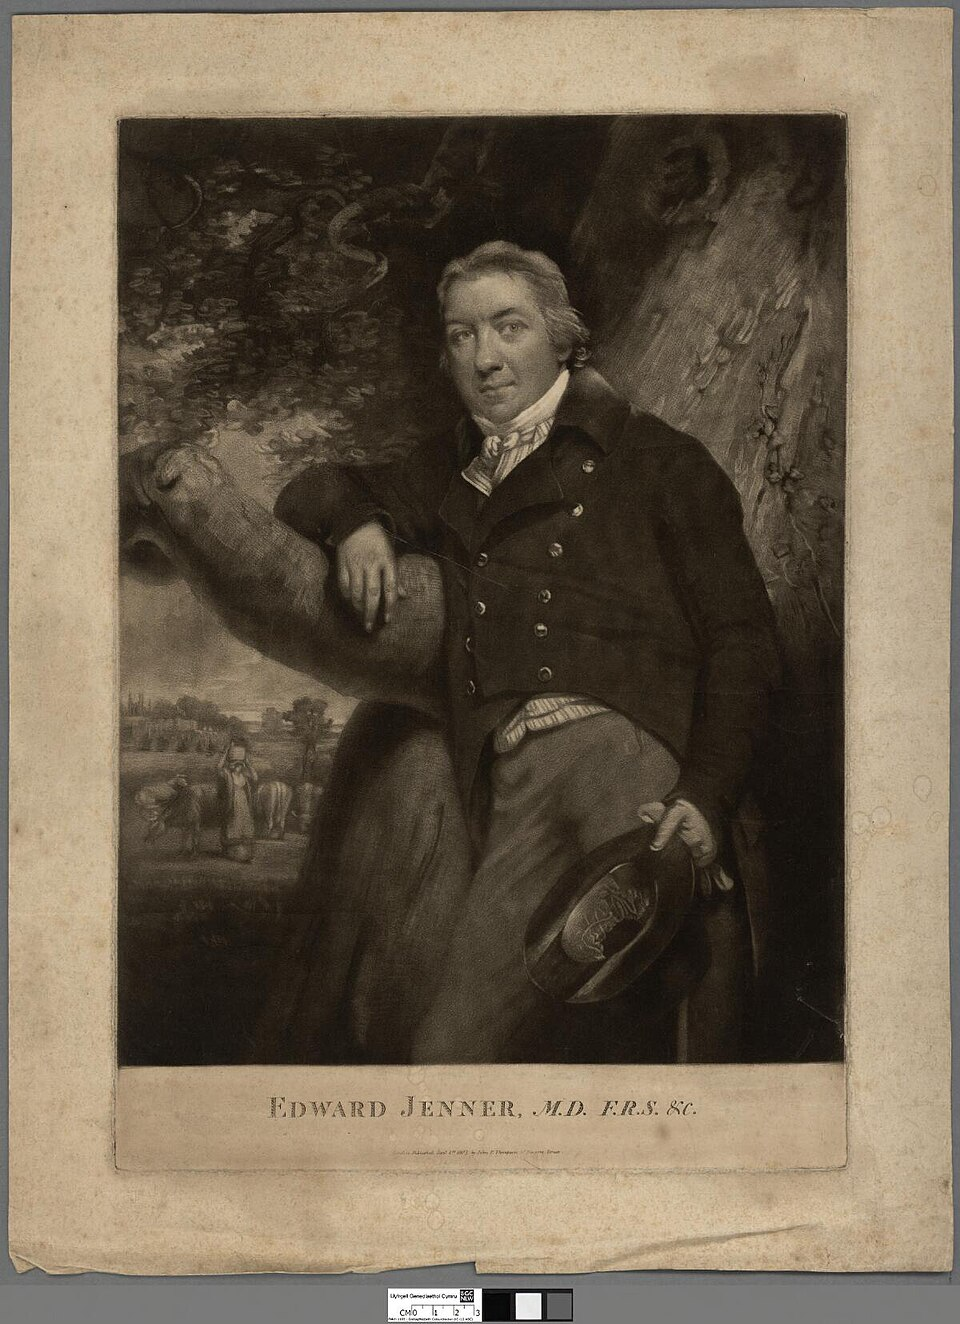
\includegraphics[width=0.30\linewidth]{images/book5/jenner.jpg}\hspace{0.04\linewidth}
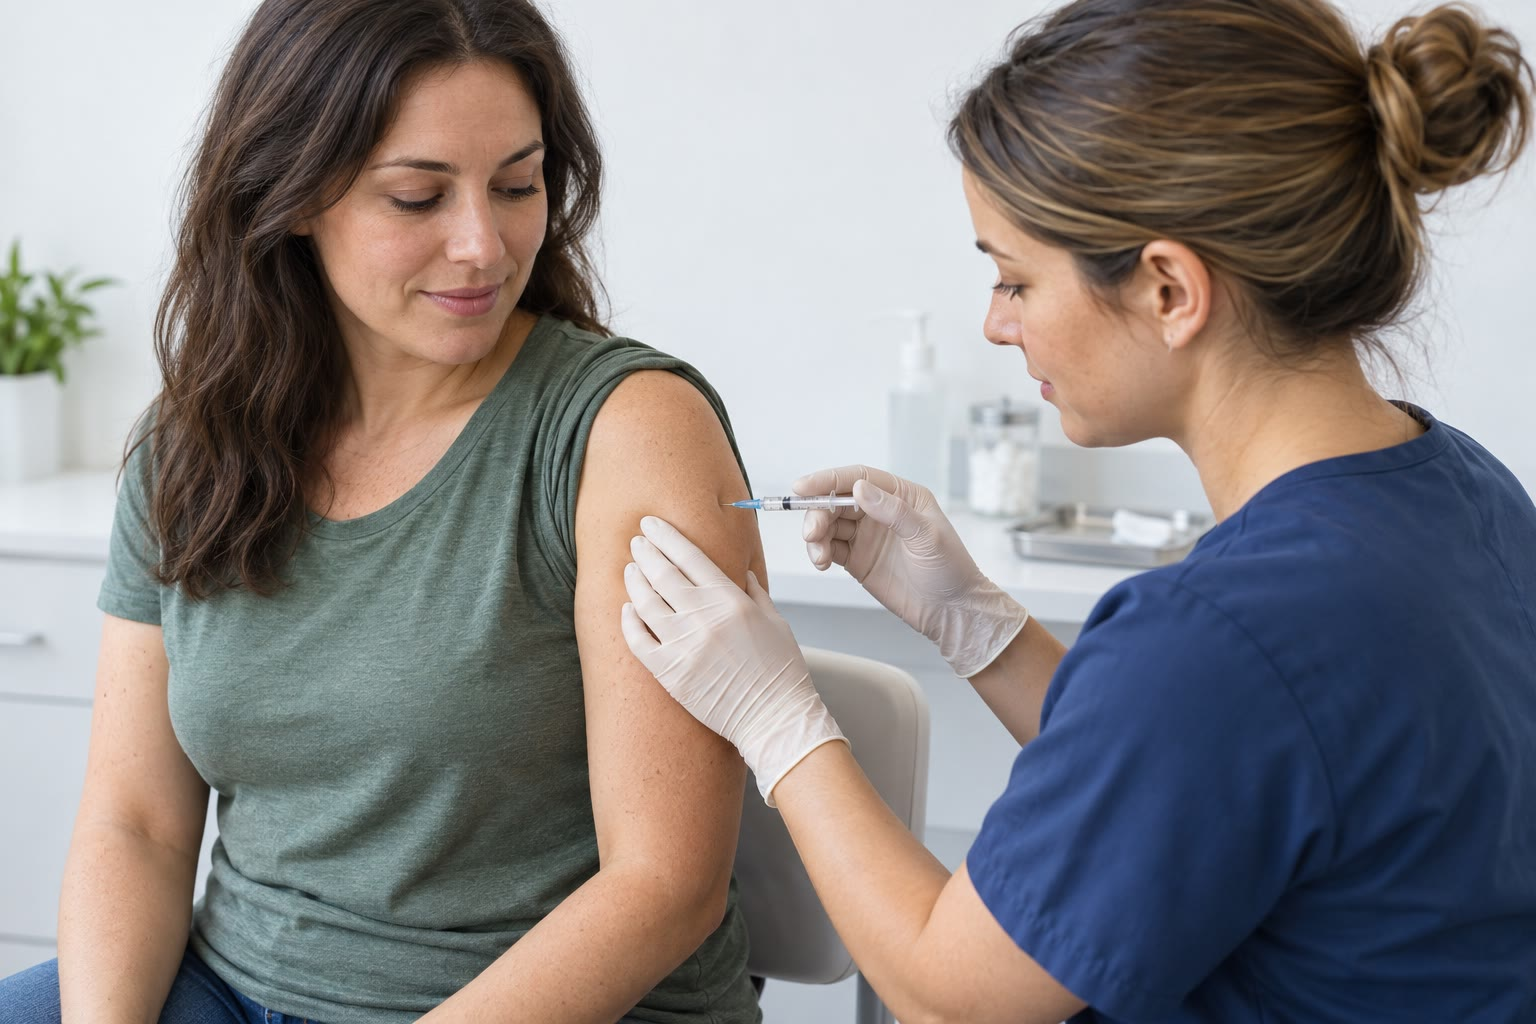
\includegraphics[width=0.50\linewidth]{images/book5/ai/b5-16-vaccination.jpg}

{\small Edward Jenner, que en 1796 protegió a un niño contra la viruela
con viruela \omterm{def:b3:adaptive-immunity:vaccine}{vacuna} y fundó la vacunación (grabado de 1807, dominio
público). Derecha: el mismo acto dos siglos después --- una \omterm{def:b3:adaptive-immunity:vaccine}{vacuna}
intramuscular, cuyo \omterm{def:b3:adaptive-immunity:lymphocytes}{antígeno} llevarán las \omterm{def:b3:innate-immunity:innate}{células dendríticas} del
deltoides a los \omterm{def:b3:adaptive-immunity:lymphocytes}{ganglios linfáticos} axilares.}
\end{omfigure}

\begin{remark}[Qué recuerda la inmunidad]\label{rem:b3:adaptive-immunity:memory}
El sistema inmunitario adaptativo es una máquina darwiniana dentro de
cada uno de nosotros: variación al azar (V(D)J, hipermutación), selección
(por el \omterm{def:b3:adaptive-immunity:lymphocytes}{antígeno}, en el \omterm{def:b3:adaptive-immunity:germinal-centre}{centro germinal}, contra lo propio en el \omterm{def:b3:adaptive-immunity:tolerance}{timo}) y
herencia (\omterm{def:b3:adaptive-immunity:response}{células de memoria}, expansión clonal). Resuelve en semanas el
problema que la evolución resuelve en milenios --- una molécula que une
una diana nunca vista --- y sus respuestas están entre los casos mejor
estudiados de evolución observada directamente. Su coste es la
\omterm{def:b3:adaptive-immunity:tolerance}{autoinmunidad}, su dependencia del juicio del sistema innato es absoluta, y
su memoria, que Jenner explotó y que las \omterm{def:b3:adaptive-immunity:vaccine}{vacunas} escriben a propósito, es
la razón de que una especie de animales longevos y de reproducción lenta
pueda sobrevivir en un mundo de microbios de reproducción rápida.
\end{remark}

\section{Ejercicios}

\begin{exercise}[$\star$]\label{exo:b3:adaptive-immunity:1}
Enúnciense los cuatro postulados de la \omterm{def:b3:adaptive-immunity:lymphocytes}{selección clonal} y el experimento
que apoya cada uno de los dos primeros.
\end{exercise}

\begin{exercise}[$\star$]\label{exo:b3:adaptive-immunity:2}
Descríbase la estructura de un \omterm{def:b3:adaptive-immunity:antibody}{anticuerpo} y dese la función de cada una
de las cinco clases.
\end{exercise}

\begin{exercise}[$\star$]\label{exo:b3:adaptive-immunity:3}
Contrástense el \omterm{def:b3:adaptive-immunity:mhc}{MHC de clase~I} y el de clase~II en distribución celular,
origen del péptido, longitud del péptido y linfocito~T que lee cada uno.
\end{exercise}

\begin{exercise}[$\star$]\label{exo:b3:adaptive-immunity:4}
Defínanse $R_{0}$ y el umbral de la \omterm{def:b3:adaptive-immunity:vaccine}{inmunidad de grupo}, y calcúlese el
umbral para las paperas ($R_{0} = 5$), la tosferina ($R_{0} = 12$) y la
gripe de 1918 ($R_{0} = 2.5$).
\end{exercise}

\begin{exercise}[$\star\star$]\label{exo:b3:adaptive-immunity:5}
Una especie tiene $V_{H} = 50$, $D = 20$, $J_{H} = 5$ y un solo locus
ligero con $V = 60$, $J = 4$. Calcúlese el repertorio combinatorio y
después el total con un factor de unión de $10^{4}$. ¿Cómo se compara con
los $10^{9}$ linfocitos~B que tiene el animal?
\end{exercise}

\begin{exercise}[$\star\star$]\label{exo:b3:adaptive-immunity:6}
La región variable de un linfocito~B de \omterm{def:b3:adaptive-immunity:germinal-centre}{centro germinal} mide
\qty{1000}{bp}; AID muta a $10^{-3}$ por par de bases y división. A lo
largo de $20$ divisiones, ¿cuántas mutaciones por célula, y entre
$10^{5}$ células cuántas variantes distintas de una sola base del
\omterm{def:b3:adaptive-immunity:antibody}{anticuerpo} se generan? Compárese con las $3000$ sustituciones simples
posibles.
\end{exercise}

\begin{exercise}[$\star\star$]\label{exo:b3:adaptive-immunity:7}
Explíquese por qué un linfocito~T de una persona no reconoce los péptidos
víricos presentados por las células de otra, y por qué ese mismo hecho
hace difíciles los trasplantes y polimórfico el sistema \omterm{def:b3:adaptive-immunity:mhc}{HLA}.
\end{exercise}

\begin{exercise}[$\star\star$]\label{exo:b3:adaptive-immunity:8}
Predígase el fenotipo inmunitario de un niño que carezca de (a) RAG1,
(b) AIRE, (c) \omterm{def:b3:adaptive-immunity:tolerance}{FoxP3}, (d) la enzima del \omterm{def:b3:adaptive-immunity:antibody}{cambio de clase} AID y (e) los
linfocitos~T CD4.
\end{exercise}

\begin{exercise}[$\star\star$]\label{exo:b3:adaptive-immunity:9}
Una \omterm{def:b3:adaptive-immunity:vaccine}{vacuna} tiene una eficacia del \qty{90}{\%} y la enfermedad
$R_{0} = 6$. ¿Qué cobertura detiene la transmisión? Si la cobertura es
del \qty{80}{\%}, ¿cuál es $R_{\text{ef}}$, y a qué fracción de la
población infecta una epidemia (úsese la relación del tamaño final con
$R_{0}$ sustituido por $R_{\text{ef}}$ entre los susceptibles --- o
arguméntese por qué eso es aproximadamente correcto)?
\end{exercise}

\begin{exercise}[$\star\star\star$]\label{exo:b3:adaptive-immunity:10}
Dedúzcase la relación del tamaño final del teorema a partir de las
ecuaciones SIR y resuélvase numéricamente para $R_{0} = 1.5$, $2$, $3$ y
$5$. ¿Por qué una epidemia no infecta nunca a todo el mundo, ni siquiera
sin intervención alguna?
\end{exercise}

\begin{exercise}[$\star\star\star$]\label{exo:b3:adaptive-immunity:11}
La \omterm{def:b3:adaptive-immunity:germinal-centre}{maduración de la afinidad} multiplica por mil la unión en tres semanas.
Trátese el \omterm{def:b3:adaptive-immunity:germinal-centre}{centro germinal} como una población bajo selección: con una
tasa de mutación de una por célula y división, una fracción $10^{-2}$ de
mutaciones que mejoran la afinidad por un factor $1.5$ y el resto
neutras o dañinas, ¿cuántas rondas de selección hacen falta para una
ganancia de mil veces, y cuántas células ha de cribar cada ronda?
Coméntese por qué el \omterm{def:b3:adaptive-immunity:germinal-centre}{centro germinal} está organizado en ciclos.
\end{exercise}

\begin{exercise}[$\star\star\star$]\label{exo:b3:adaptive-immunity:12}
Las enfermedades autoinmunitarias son más frecuentes en las mujeres y se
asocian a alelos \omterm{def:b3:adaptive-immunity:mhc}{HLA}; la diabetes de tipo~1 se ha quintuplicado en
cincuenta años en los países ricos. Propónganse, con los mecanismos de
este capítulo y del \cref{ch:b3:microbiomes}, explicaciones de cada
observación y una prueba de cada una.
\end{exercise}

\section{Problema: una campaña de vacunación}

\begin{problem}[{Problema de fin de semana --- un repertorio contado, una
respuesta cronometrada desde cien células hasta un mililitro de suero, un
centro germinal ejecutado como algoritmo evolutivo y una campaña de
sarampión planeada frente al umbral de grupo, hasta llegar al tamaño del
repertorio, al anticuerpo que fabrica en un día una célula plasmática y a
la cobertura que necesita un país}]
\label{pb:b3:adaptive-immunity:1}
Datos: $V_{H} = 40$, $D = 25$, $J_{H} = 6$; loci ligeros $(40, 5)$ y
$(30, 4)$; factor de unión $3\times 10^{4}$. Un cuerpo tiene $10^{11}$
linfocitos~B; uno de cada $10^{5}$ une un epítopo dado; se reclutan $100$
precursores; una división cada \qty{8}{h} durante $7$ días; el
\qty{30}{\%} del clon pasa a ser \omterm{def:b3:adaptive-immunity:response}{células plasmáticas} que secretan $2000$
moléculas de IgG por segundo cada una; la IgG mide \qty{150}{kDa};
volumen plasmático \qty{3}{L}; semivida de la IgG, \qty{21}{d}. \omterm{def:b3:adaptive-immunity:germinal-centre}{Centro
germinal}: región variable de \qty{1000}{bp}, $10^{-3}$ mutaciones por bp
y división, y una de cada $100$ mutaciones mejora la afinidad por $1.5$.
Sarampión: $R_{0} = 15$, \omterm{def:b3:adaptive-immunity:vaccine}{eficacia vacunal} $0.93$ tras una dosis y $0.97$
tras dos; un país de $5\times 10^{6}$ habitantes con $60\,000$
nacimientos al año.

\medskip
\noindent\textbf{Parte I --- El repertorio.}
\begin{enumerate}
  \item Calcúlense el repertorio combinatorio y el total con la
        \omterm{def:b3:adaptive-immunity:antibody}{diversidad de unión}.
  \item Compárese con el número de linfocitos~B. ¿Qué fracción del
        repertorio posible expresa un cuerpo a la vez, y qué se sigue de
        ello para los repertorios de dos individuos?
  \item ¿Cuántos linfocitos~B del cuerpo unen el epítopo? ¿Cuántos, en
        promedio, en un \omterm{def:b3:adaptive-immunity:lymphocytes}{ganglio linfático} con $10^{8}$ linfocitos~B?
  \item Un recién nacido tiene $10^{9}$ linfocitos~B. ¿Cuántos unen el
        epítopo, y por qué es débil su respuesta aun así?
  \item El tercer bucle de la cadena pesada de un \omterm{def:b3:adaptive-immunity:antibody}{anticuerpo} lo fabrica
        la \omterm{def:b3:adaptive-immunity:antibody}{diversidad de unión}. Explíquese por qué ese bucle es la parte
        más variable de la molécula y suele estar en el centro del sitio
        de unión.
  \item La \omterm{def:b3:adaptive-immunity:germinal-centre}{hipermutación somática} añade diversidad después de la
        selección y la V(D)J antes. ¿Por qué conviene tener las dos, en
        ese orden?
\end{enumerate}

\medskip
\noindent\textbf{Parte II --- La respuesta.}
\begin{enumerate}[resume]
  \item A partir de $100$ células que se dividen cada \qty{8}{h},
        ¿cuántas hay al cabo de $7$ días? ¿Cuántas \omterm{def:b3:adaptive-immunity:response}{células plasmáticas}?
  \item ¿Cuántas moléculas de IgG secretan al día, y qué masa? ¿Qué
        concentración sérica da la producción de un día en \qty{3}{L}?
  \item Tras diez días de secreción a ese ritmo, y sin contar la
        degradación, ¿cuál es la concentración en g/L? Compárese con la
        IgG total normal de \qty{10}{g/L}.
  \item Las \omterm{def:b3:adaptive-immunity:response}{células plasmáticas} mueren al cabo de dos semanas; el
        \omterm{def:b3:adaptive-immunity:antibody}{anticuerpo} decae entonces con semivida \qty{21}{d}. ¿Cuánto tarda
        la concentración de la pregunta 9 en caer cien veces? ¿Qué
        mantiene el \omterm{def:b3:adaptive-immunity:antibody}{anticuerpo} durante años?
  \item Una respuesta secundaria parte de $10^{5}$ \omterm{def:b3:adaptive-immunity:response}{células de memoria}.
        ¿Cuántas células hay al cabo de $3$ días, y cómo se compara eso
        con la respuesta primaria en el día 3 y en el día 7?
  \item Explíquese por qué la IgM llega primero y la IgG después en una
        respuesta primaria, y por qué la respuesta secundaria es IgG
        desde el principio.
\end{enumerate}

\medskip
\noindent\textbf{Parte III --- El \omterm{def:b3:adaptive-immunity:germinal-centre}{centro germinal}.}
\begin{enumerate}[resume]
  \item ¿Cuántas mutaciones adquiere un linfocito~B en su región variable
        por división? ¿Y a lo largo de $20$ divisiones?
  \item ¿Qué fracción de las hijas de una división lleva una mutación que
        mejora? En un \omterm{def:b3:adaptive-immunity:germinal-centre}{centro germinal} de $10^{4}$ células en división,
        ¿cuántas células mejoradas aparecen por división?
  \item ¿Cuántas mejoras sucesivas de $1.5$ dan una ganancia de mil veces
        en afinidad? Si cada ronda de selección cuesta dos divisiones
        (\qty{12}{h}), ¿cuánto tiempo es eso?
  \item La mayoría de las mutaciones estropean el \omterm{def:b3:adaptive-immunity:antibody}{anticuerpo}. Si el
        \qty{50}{\%} de las mutaciones destruyen la unión, ¿qué fracción
        de células sobrevive a la mutación de cada división, y por qué ha
        de matar la zona clara a la mayoría de las células?
  \item Una \omterm{def:b3:adaptive-immunity:vaccine}{vacuna} administrada en dos dosis separadas seis semanas
        rinde \omterm{def:b3:adaptive-immunity:antibody}{anticuerpos} de más afinidad que una sola dosis.
        Explíquese con el \omterm{def:b3:adaptive-immunity:germinal-centre}{centro germinal}.
  \item Algunos \omterm{def:b3:virology:virus}{virus} (el VIH, la gripe) escapan a los \omterm{def:b3:adaptive-immunity:antibody}{anticuerpos}
        mutando su superficie. Explíquese por qué el \omterm{def:b3:adaptive-immunity:germinal-centre}{centro germinal} es
        pese a todo la base de la esperanza de una \omterm{def:b3:adaptive-immunity:vaccine}{vacuna} que proteja
        ampliamente.
\end{enumerate}

\medskip
\noindent\textbf{Parte IV --- La campaña.}
\begin{enumerate}[resume]
  \item Umbral de grupo del sarampión y cobertura necesaria con una
        dosis; y con dos dosis.
  \item El país \omterm{def:b3:adaptive-immunity:vaccine}{vacuna} con dos dosis al \qty{90}{\%} de los niños.
        Fracción inmune, $R_{\text{ef}}$ y veredicto: ¿circula el
        sarampión?
  \item ¿Cuántos niños susceptibles se acumulan por año de nacimientos
        con una cobertura del \qty{90}{\%} (los no vacunados más los
        fallos vacunales)? Tras cinco años sin sarampión, ¿cuántos
        susceptibles hay, y por qué una importación provoca entonces un
        brote?
  \item Úsese la relación del tamaño final con el número reproductivo
        efectivo entre los susceptibles para estimar a qué fracción de
        esos susceptibles infecta un brote. (Tómese el
        $R_{\text{ef}}$ de la pregunta 20 como número reproductivo de
        toda la población, y nótese que dentro de la reserva susceptible
        la enfermedad se propaga como si $R_{0}$ fuera
        $R_{\text{ef}}$.)
  \item La cobertura sube al \qty{95}{\%} con dos dosis. Fracción inmune
        y $R_{\text{ef}}$; ¿se cumple el umbral?
  \item Los lactantes menores de un año no pueden vacunarse contra el
        sarampión y son los que más probablemente mueren por él.
        Explíquese cómo los protege la campaña, y qué le ocurre a esa
        protección si la cobertura baja al \qty{85}{\%}.
  \item Resúmase: el repertorio total (pregunta~1), la IgG que fabrican
        en un día las \omterm{def:b3:adaptive-immunity:response}{células plasmáticas} (pregunta~8) y la cobertura de
        dos dosis que necesita el país (pregunta~19).
\end{enumerate}
\end{problem}
